%!TEX root = ../../super_main.tex

\section{Automated Unit Test}
\label{sec:automated_unit_test}

\todo[inline]{Rikke: Er ikke helt sikker på at jeg kan følge processen her. Hvordan har I lavet integrations test og hvordan med black box test?}
Our development method states that all code we develop should be made in a test-first fashion (see \secref{sec:extreme_programming}). We therefore attempted to always make unit tests for all the features we implemented. In some cases it was not possible to create dynamic white box unit tests, and we therefore, in these cases, switched to a dynamic black box approach, where we made test specifications, executed some part of the code manually and observed the result relative to the specification. We mainly did this for the more complex parts of the code, for example the \mono{BackgroundSensorService} class, which schedules all the \mono{SensorProvider}s asynchronously and sends the results to the server. We also did this for tests on a higher level, such as integration tests, which means that the combinations of our different modules only have manual tests to confirm that they work together. This results in a code coverage from the unit tests that are lower than expected, but we can confirm with manual tests that the behavior is as expected. 
\\\\
Our code coverage graphs can be seen in \figref{fig:android_project_code_coverage} and \figref{fig:php_project_code_coverage}, for our Android and PHP projects respectively. The two figures are different because we use different plugins on the CI server. We have not used a more strict testing metric than line coverage, due to limited time. We can therefore not guarantee that all things such as branches, exceptions, etc, are tested in the code, but we can guarantee that it is possible to run most of our code successfully. In the android project our line coverage percentage is 43\%, which is rather low. But as explained previously, this is due to the complexity of the integration tests which were manual instead. 

% In \figref{fig:android_project_code_coverage} the line coverage is represented with green while missed lines are represented with red. In \figref{fig:php_project_code_coverage} the red line is method coverage, blue is line coverage and green is total.

\begin{figure}[!htbp]
    \centering
    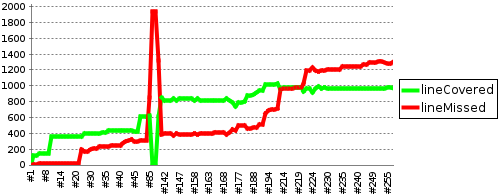
\includegraphics[width=0.7\textwidth]{graphic/quality_assurance/jenkins_android_code_coverage}
    \caption{Android project code coverage}
    \label{fig:android_project_code_coverage}
\end{figure}
\FloatBarrier

\noindent
In the PHP project, we have a 74\% line coverage, which is rather good. Most of the untested code is library- or auto generated code, and we have not tested this because we assume these parts work as they are supposed to. This is a risk management assessment we have made, and deemed insignificant, in contrast to the speed we gain from using the libraries without testing them. % If we only considered coverage on the code we made ourselves, it would probably exceed 90\%. 

\begin{figure}[!htbp]
    \centering
    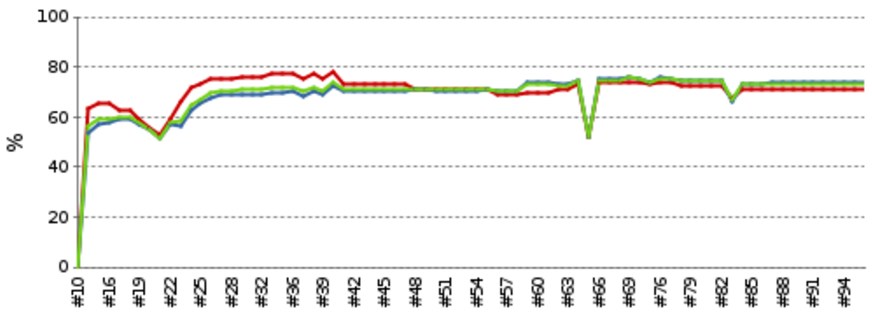
\includegraphics[width=0.7\textwidth]{graphic/quality_assurance/jenkins_php_code_coverage}
    \caption{PHP project code coverage}
    \label{fig:php_project_code_coverage}
\end{figure}
\FloatBarrier